\subsection{Überblick}
DYCOS (\underline{DY}namic \underline{C}lassification algorithm with
c\underline{O}ntent and \underline{S}tructure) ist ein
Knotenklassifizierungsalgorithmus, der Ursprünglich in \cite{aggarwal2011}
vorgestellt wurde.

Ein zentrales Element des DYCOS-Algorithmus ist der sog. {\it Random Walk}:

\begin{definition}[Random Walk, Sprung]
    Sei $G = (V, E)$ mit $E \subseteq V \times V$ ein Graph und
    $v_0 \in V$ ein Knoten des Graphen.

    Ein Random Walk der Länge $l$ auf $G$, startend bei $v_0$ ist nun der
    zeitdiskrete stochastische Prozess, der $v_i$ auf einen zufällig gewählten
    Nachbarn $v_{i+1}$ abbildet (für $i \in 0, \dots, l-1$). Die Abbildung $v_i
    \mapsto v_{i+1}$ heißt ein Sprung.
\end{definition}

Der DYCOS-Algorithmus klassifiziert einzelne Knoten, indem $r$ Random Walks der
Länge $l$, startend bei dem zu klassifizierenden Knoten $v$ gemacht werden.
Dabei werden die Beschriftungen der besuchten Knoten gezählt. Die Beschriftung,
die am häufigsten vorgekommen ist, wird als Beschriftung für $v$ gewählt. DYCOS
nutzt also die sog. Homophilie, d.~h. die Eigenschaft, dass Knoten, die nur
wenige Hops von einander entfernt sind, häufig auch ähnlich sind \cite{bhagat}.
Der DYCOS-Algorithmus arbeitet jedoch nicht direkt auf dem Graphen, sondern
erweitert ihn mit Hilfe der zur Verfügung stehenden Texte. Wie diese
Erweiterung erstellt wird, wird im Folgenden erklärt.\\
Für diese Erweiterung wird zuerst wird Vokabular $W_t$ bestimmt, das
charakteristisch für eine Knotengruppe ist. Wie das gemacht werden kann und
warum nicht einfach jedes Wort in das Vokabular aufgenommen wird, wird in
\cref{sec:vokabularbestimmung} erläutert.\\
Nach der Bestimmung des Vokabulars wird für jedes Wort im Vokabular ein
Wortknoten zum Graphen hinzugefügt. Alle Knoten, die der Graph zuvor hatte,
werden nun \enquote{Strukturknoten} genannt.
Ein Strukturknoten $v$ wird genau dann mit einem Wortknoten $w \in W_t$
verbunden, wenn $w$ in einem Text von $v$ vorkommt. \Cref{fig:erweiterter-graph}
zeigt beispielhaft den so entstehenden, semi-bipartiten Graphen.
Der DYCOS-Algorithmus betrachtet also die Texte, die einem Knoten
zugeordnet sind, als eine Multimenge von Wörtern. Das heißt, zum einen
wird nicht auf die Reihenfolge der Wörter geachtet, zum anderen wird
bei Texten eines Knotens nicht zwischen verschiedenen
Texten unterschieden. Jedoch wird die Anzahl der Vorkommen
jedes Wortes berücksichtigt.

\begin{figure}[htp]
    \centering
    \tikzstyle{vertex}=[draw,black,circle,minimum size=10pt,inner sep=0pt]
\tikzstyle{edge}=[very thick]
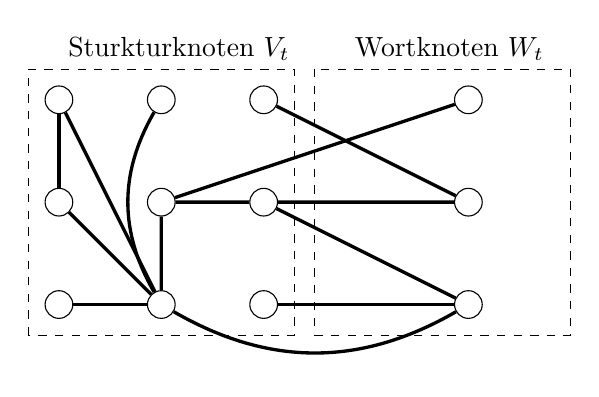
\begin{tikzpicture}[scale=1.3]
    \node (a)[vertex] at (0,0) {};
    \node (b)[vertex]  at (0,1) {};
    \node (c)[vertex] at (0,2) {};
    \node (d)[vertex] at (1,0) {};
    \node (e)[vertex]  at (1,1) {};
    \node (f)[vertex] at (1,2) {};
    \node (g)[vertex] at (2,0) {};
    \node (h)[vertex] at (2,1) {};
    \node (i)[vertex] at (2,2) {};

    \node (x)[vertex] at (4,0) {};
    \node (y)[vertex] at (4,1) {};
    \node (z)[vertex] at (4,2) {};

    \draw[edge] (a) -- (d);
    \draw[edge] (b) -- (d);
    \draw[edge] (b) -- (c);
    \draw[edge] (c) -- (d);
    \draw[edge] (d) -- (e);
    \draw[edge] (d) edge[bend left] (f);
    \draw[edge] (d) edge[bend right] (x);
    \draw[edge] (g) edge (x);
    \draw[edge] (h) edge (x);
    \draw[edge] (h) edge (y);
    \draw[edge] (h) edge (e);
    \draw[edge] (e) edge (z);
    \draw[edge] (i) edge (y);

    \draw [dashed] (-0.3,-0.3) rectangle (2.3,2.3);
    \draw [dashed] (2.5,2.3) rectangle (5, -0.3);

    \node (struktur)[label={[label distance=0cm]0:Sturkturknoten $V_t$}] at (-0.1,2.5) {};
    \node (struktur)[label={[label distance=0cm]0:Wortknoten $W_t$}] at (2.7,2.5) {};
\end{tikzpicture}

    \caption{Erweiterter Graph}
    \label{fig:erweiterter-graph}
\end{figure}

Entsprechend werden zwei unterschiedliche Sprungtypen unterschieden, die
strukturellen Sprünge und inhaltliche Zweifachsprünge:

\begin{definition}[struktureller Sprung]
    Sei $G_{E,t} = (V_t, E_{S,t} \cup E_{W,t}, V_{L,t}, W_{t})$ der
    um die Wortknoten $W_{t}$ erweiterte Graph.

    Dann heißt das zufällige wechseln des aktuell betrachteten
    Knoten $v \in V_t$ zu einem benachbartem Knoten $w \in V_t$
    ein \textit{struktureller Sprung}.
\end{definition}
\goodbreak
Im Gegensatz dazu benutzten inhaltliche Zweifachsprünge tatsächlich die
Grapherweiterung:
\begin{definition}[inhaltlicher Zweifachsprung]
    Sei $G_t = (V_t, E_{S,t} \cup E_{W,t}, V_{L,t}, W_{t})$ der um die
    Wortknoten $W_{t}$ erweiterte Graph.

    Dann heißt das zufällige wechseln des aktuell betrachteten Knoten $v \in
    V_t$ zu einem benachbartem Knoten $w \in W_t$ und weiter zu einem
    zufälligem Nachbar $v' \in V_t$ von $w$ ein inhaltlicher Zweifachsprung.
\end{definition}

Jeder inhaltliche Zweifachsprung beginnt und endet also in einem
Strukturknoten, springt über einen Wortknoten und ist ein Pfad der Länge~2.

Ob in einem Sprung der Random Walks ein struktureller Sprung oder ein
inhaltlicher Zweifachsprung gemacht wird, wird jedes mal zufällig neu
entschieden. Dafür wird der Parameter $0 \leq p_S \leq 1$ für den Algorithmus
gewählt. Mit einer Wahrscheinlichkeit von $p_S$ wird ein struktureller Sprung
durchgeführt und mit einer Wahrscheinlichkeit von $(1-p_S)$ ein modifizierter
inhaltlicher Zweifachsprung, wie er in \cref{sec:sprungtypen} erklärt wird,
gemacht. Der Parameter $p_S$ gibt an, wie wichtig die Struktur des Graphen im
Verhältnis zu den textuellen Inhalten ist. Bei $p_S = 0$ werden ausschließlich
die Texte betrachtet, bei $p_S = 1$ ausschließlich die Struktur des Graphen.

Die Vokabularbestimmung kann zu jedem Zeitpunkt $t$ durchgeführt werden, muss
es aber nicht.

In \cref{alg:DYCOS} steht der DYCOS-Algorithmus in Form von Pseudocode:
In \cref{alg1:l8} wird für jeden unbeschrifteten Knoten
durch die folgenden Zeilen eine Beschriftung gewählt.

\Cref{alg1:l10} führt $r$ Random Walks durch. In \cref{alg1:l11} wird eine
temporäre Variable für den aktuell betrachteten Knoten angelegt.

In \cref{alg1:l12} bis \cref{alg1:l21} werden einzelne Random Walks der Länge
$l$ durchgeführt, wobei die beobachteten Beschriftungen gezählt werden und mit
einer Wahrscheinlichkeit von $p_S$ ein struktureller Sprung durchgeführt wird.

\begin{algorithm}[ht]
    \begin{algorithmic}[1]
        \Require \\$G_{E,t} = (V_t, E_{S,t} \cup E_{W,t}, V_{L,t}, W_t)$ (Erweiterter Graph),\\
                 $r$ (Anzahl der Random Walks),\\
                 $l$ (Länge eines Random Walks),\\
                 $p_s$ (Wahrscheinlichkeit eines strukturellen Sprungs),\\
                 $q$ (Anzahl der betrachteten Knoten in der Clusteranalyse)
        \Ensure  Klassifikation von $V_t \setminus V_{L,t}$\\
        \\

        \ForAll{Knoten $v \in V_t \setminus V_{L,t}$}\label{alg1:l8}
            \State $d \gets $ leeres assoziatives Array
            \For{$i = 1, \dots,r$}\label{alg1:l10}
                \State $w \gets v$\label{alg1:l11}
                \For{$j= 1, \dots, l$}\label{alg1:l12}
                    \State $sprungTyp \gets \Call{random}{0, 1}$
                    \If{$sprungTyp \leq p_S$}
                        \State $w \gets$ \Call{SturkturellerSprung}{$w$}
                    \Else
                        \State $w \gets$ \Call{InhaltlicherZweifachsprung}{$w$}
                    \EndIf
                    \State $beschriftung \gets w.\Call{GetLabel}{ }$
                    \If{$!d.\Call{hasKey}{beschriftung}$}
                        \State $d[beschriftung] \gets 0$
                    \EndIf
                    \State $d[beschriftung] \gets d[beschriftung] + 1$
                \EndFor\label{alg1:l21}
            \EndFor

            \If{$d$.\Call{isEmpty}{ }} \Comment{Es wurde kein beschrifteter Knoten gesehen}
                \State $M_H \gets \Call{HäufigsteLabelImGraph}{ }$
            \Else
                \State $M_H \gets \Call{max}{d}$
            \EndIf
            \\
            \State \Comment{Wähle aus der Menge der häufigsten Beschriftungen $M_H$ zufällig eine aus}
            \State $label \gets \Call{Random}{M_H}$
            \State $v.\Call{AddLabel}{label}$ \Comment{und weise dieses $v$ zu}
        \EndFor
        \State \Return Beschriftungen für $V_t \setminus V_{L,t}$
    \end{algorithmic}
\caption{DYCOS-Algorithmus}
\label{alg:DYCOS}
\end{algorithm}

\subsection{Datenstrukturen}
Zusätzlich zu dem gerichteten Graphen $G_t = (V_t, E_t, V_{L,t})$ verwaltet der
DYCOS-Algorithmus zwei weitere Datenstrukturen:
\begin{itemize}
    \item Für jeden Knoten $v \in V_t$ werden die vorkommenden Wörter,
          die auch im Vokabular $W_t$ sind,
          und deren Anzahl gespeichert. Das könnte z.~B. über ein
          assoziatives Array (auch \enquote{dictionary} oder
            \enquote{map} genannt) geschehen. Wörter, die nicht in
          Texten von $v$ vorkommen, sind nicht im Array. Für
          alle vorkommenden Wörter ist der gespeicherte Wert zum
          Schlüssel $w \in W_t$ die Anzahl der Vorkommen von
          $w$ in den Texten von $v$.
    \item Für jedes Wort des Vokabulars $W_t$ wird eine Liste von
          Knoten verwaltet, in deren Texten das Wort vorkommt.
          Diese Liste wird bei den inhaltlichen Zweifachsprung,
          der in \cref{sec:sprungtypen} erklärt wird,
          verwendet.
\end{itemize}

\subsection{Sprungtypen}\label{sec:sprungtypen}
Die beiden bereits definierten Sprungtypen, der strukturelle Sprung sowie der
inhaltliche Zweifachsprung werden im Folgenden erklärt.
\goodbreak
Der strukturelle Sprung entspricht einer zufälligen Wahl eines Nachbarknotens,
wie es in \cref{alg:DYCOS-structural-hop} gezeigt wird.
\begin{algorithm}[H]
    \begin{algorithmic}[1]
        \Procedure{SturkturellerSprung}{Knoten $v$, Anzahl $q$}
            \State $n \gets v.\Call{NeighborCount}{}$ \Comment{Wähle aus der Liste der Nachbarknoten}
            \State $r \gets \Call{RandomInt}{0, n-1}$ \Comment{einen zufällig aus}
            \State $v \gets v.\Call{Next}{r}$ \Comment{Gehe zu diesem Knoten}
            \State \Return $v$
        \EndProcedure
    \end{algorithmic}
\caption{Struktureller Sprung}
\label{alg:DYCOS-structural-hop}
\end{algorithm}

Bei inhaltlichen Zweifachsprüngen ist jedoch nicht sinnvoll so strikt nach der
Definition vorzugehen,  also direkt von einem strukturellem Knoten $v \in V_t$
zu einem mit $v$ verbundenen Wortknoten $w \in W_t$ zu springen und von diesem
wieder zu einem verbundenem strukturellem Knoten $v' \in V_t$. Würde dies
gemacht werden, wäre zu befürchten, dass aufgrund von Homonymen die Qualität der
Klassifizierung verringert wird. So hat \enquote{Brücke} im Deutschen viele
Bedeutungen. Gemeint sein können z.~B. das Bauwerk, das Entwurfsmuster der
objektorientierten Programmierung oder ein Teil des Gehirns.

Deshalb wird für jeden Knoten $v$, von dem aus ein inhaltlicher
Zweifachsprung gemacht werden soll folgende Textanalyse durchgeführt:
\begin{enumerate}[label=C\arabic*,ref=C\arabic*]
    \item \label{step:c1} Gehe alle in $v$ startenden Random Walks der Länge $2$ durch
          und erstelle eine Liste $L$ der erreichbaren Knoten $v'$. Speichere
          außerdem, durch wie viele Pfade diese Knoten $v'$ jeweils erreichbar
          sind.
    \item \label{step:c2} Betrachte im Folgenden nur die Top-$q$ Knoten bzgl.
          der Anzahl der Pfade von $v$ nach $v'$, wobei $q \in \mathbb{N}$
          eine zu wählende Konstante des DYCOS-Algorithmus ist.\footnote{Sowohl für den DBLP, als auch für den
CORA-Datensatz wurde in \cite[S. 364]{aggarwal2011} $q=10$ gewählt.}
          Diese Knotenmenge heiße im Folgenden $T(v)$ und $p(v, v')$ sei die
          Anzahl der Pfade von $v$ über einen Wortknoten nach $v'$.
    \item \label{step:c3} Wähle mit Wahrscheinlichkeit
          $\frac{p(v, v')}{\sum_{w \in T(v)} p(v, w)}$ den Knoten $v' \in T(v)$
          als Ziel des Zweifachsprungs.
\end{enumerate}

Konkret könnte also ein inhaltlicher Zweifachsprung sowie wie in
\cref{alg:DYCOS-content-multihop} beschrieben umgesetzt werden.
Der Algorithmus bekommt einen Startknoten $v \in V_T$ und
einen $q \in \mathbb{N}$ als Parameter. $q$ ist ein Parameter der
für den DYCOS-Algorithmus zu wählen ist. Dieser Parameter beschränkt
die Anzahl der möglichen Zielknoten $v' \in V_T$ auf diejenigen
$q$ Knoten, die $v$ bzgl. der Textanalyse am ähnlichsten sind.

In \cref{alg:l2} bis \cref{alg:l5} wird \cref{step:c1} durchgeführt und alle
erreichbaren Knoten in $reachableNodes$ mit der Anzahl der Pfade, durch die sie
erreicht werden können, gespeichert.

In \cref{alg:l6} wird \cref{step:c2} durchgeführt. Ab hier gilt
\[ |T| = \begin{cases}q               &\text{falls } |reachableNodes|\geq q\\
                     |reachableNodes| &\text{sonst }\end{cases}\]

Bei der Wahl der Datenstruktur von $T$ ist zu beachten, dass man in
\cref{alg:21} über Indizes auf Elemente aus $T$ zugreifen können muss.

In \cref{alg:l8} bis \ref{alg:l13} wird ein assoziatives Array erstellt, das
von $v' \in T(v)$ auf die relative Häufigkeit bzgl. aller Pfade von $v$ zu
Knoten aus den Top-$q$ abbildet.

In allen folgenden Zeilen wird \cref{step:c3} durchgeführt. In \cref{alg:15}
bis \cref{alg:22} wird ein Knoten $v' \in T(v)$ mit einer Wahrscheinlichkeit,
die seiner relativen Häufigkeit am Anteil der Pfaden der Länge 2 von $v$ nach
$v'$ über einen beliebigen Wortknoten entspricht ausgewählt und schließlich
zurückgegeben.

\begin{algorithm}
  \caption{Inhaltlicher Zweifachsprung}
  \label{alg:DYCOS-content-multihop}
    \begin{algorithmic}[1]
        \Procedure{InhaltlicherZweifachsprung}{Knoten $v \in V_T$, $q \in \mathbb{N}$}
            \State $erreichbareKnoten \gets$ leeres assoziatives Array\label{alg:l2}
            \ForAll{Wortknoten $w$ in $v.\Call{getWordNodes}{ }$}
                \ForAll{Strukturknoten $x$ in $w.\Call{getStructuralNodes}{ }$}
                    \If{$!erreichbareKnoten.\Call{hasKey}{x}$}
                        \State $erreichbareKnoten[x] \gets 0$
                    \EndIf
                    \State $erreichbareKnoten[x] \gets erreichbareKnoten[x] + 1$
                \EndFor
            \EndFor\label{alg:l5}
            \State \label{alg:l6} $T \gets \Call{max}{erreichbareKnoten, q}$
            \\
            \State \label{alg:l8} $s \gets 0$
            \ForAll{Knoten $x \in T$}
                \State $s \gets s + erreichbareKnoten[x]$
            \EndFor
            \State $relativeHaeufigkeit \gets $ leeres assoziatives Array
            \ForAll{Knoten $x \in T$}
                \State $relativeHaeufigkeit \gets \frac{erreichbareKnoten[x]}{s}$
            \EndFor\label{alg:l13}
            \\
            \State \label{alg:15} $random \gets \Call{random}{0, 1}$
            \State $r \gets 0.0$
            \State $i \gets 0$
            \While{$s < random$}
                \State $r \gets r + relativeHaeufigkeit[i]$
                \State $i \gets i + 1$
            \EndWhile

            \State $v \gets T[i-1]$ \label{alg:21}
            \State \Return $v$ \label{alg:22}
        \EndProcedure
    \end{algorithmic}
\end{algorithm}

\subsection{Vokabularbestimmung}\label{sec:vokabularbestimmung}
Da die Größe des Vokabulars die Datenmenge signifikant beeinflusst,
liegt es in unserem Interesse so wenig Wörter wie möglich ins
Vokabular aufzunehmen. Insbesondere sind Wörter nicht von Interesse,
die in fast allen Texten vorkommen, wie im Deutschen z.~B.
\enquote{und}, \enquote{mit} und die Pronomen. Es ist wünschenswert Wörter zu
wählen, die die Texte möglichst stark voneinander Unterscheiden. Der
DYCOS-Algorithmus wählt die Top-$m$ dieser Wörter als Vokabular, wobei
$m \in \mathbb{N}$ eine festzulegende Konstante ist. In \cite[S. 365]{aggarwal2011}
wird der Einfluss von $m \in \Set{5,10, 15,20}$ auf die Klassifikationsgüte
untersucht und festgestellt, dass die Klassifikationsgüte mit größerem $m$
sinkt, sie also für $m=5$ für den DBLP-Datensatz am höchsten ist. Für den
CORA-Datensatz wurde mit $m \in \set{3,4,5,6}$ getestet und kein signifikanter
Unterschied festgestellt.

Nun kann man manuell eine Liste von zu beachtenden Wörtern erstellen
oder mit Hilfe des Gini-Koeffizienten automatisch ein Vokabular erstellen.
Der Gini-Koeffizient ist ein statistisches Maß, das die Ungleichverteilung
bewertet. Er ist immer im Intervall $[0,1]$, wobei $0$ einer
Gleichverteilung entspricht und $1$ der größtmöglichen Ungleichverteilung.

Sei nun $n_i(w)$ die Häufigkeit des Wortes $w$ in allen Texten mit der $i$-ten
Knotenbeschriftung.
\begin{align}
    p_i(w) &:= \frac{n_i(w)}{\sum_{j=1}^{|\L_t|} n_j(w)} &\text{(Relative Häufigkeit des Wortes $w$)}\\
    G(w)   &:= \sum_{j=1}^{|\L_t|} p_j(w)^2              &\text{(Gini-Koeffizient von $w$)}
\end{align}
In diesem Fall ist $G(w)=0$ nicht möglich, da zur Vokabularbestimmung nur
Wörter betrachtet werden, die auch vorkommen.

Ein Vorschlag, wie die Vokabularbestimmung implementiert werden kann, ist als
Pseudocode mit \cref{alg:vokabularbestimmung} gegeben. In \cref{alg4:l6} wird
eine Teilmenge $S_t \subseteq V_{L,t}$ zum Generieren des Vokabulars gewählt.
In \cref{alg4:l8} wird ein Array $cLabelWords$ erstellt, das $(|\L_t|+1)$
Felder hat. Die Elemente dieser Felder sind jeweils assoziative Arrays, deren
Schlüssel Wörter und deren Werte natürliche Zahlen sind. Die ersten $|\L_t|$
Elemente von $cLabelWords$ dienen dem Zählen der Häufigkeit der Wörter von
Texten aus $S_t$, wobei für jede Beschriftung die Häufigkeit einzeln gezählt
wird. Das letzte Element aus $cLabelWords$ zählt die Summe der Wörter. Diese
Datenstruktur wird in \cref{alg4:l10} bis \ref{alg4:l12} gefüllt.

In \cref{alg4:l17} bis \ref{alg4:l19} wird die relative Häufigkeit der Wörter
bzgl. der Beschriftungen bestimmt. Daraus wird in \cref{alg4:l20} bis
\ref{alg4:l22} der Gini-Koeffizient berechnet. Schließlich werden in
\cref{alg4:l23} bis \ref{alg4:l24} die Top-$q$ Wörter mit den
höchsten Gini-Koeffizienten zurückgegeben.

\begin{algorithm}[ht]
    \begin{algorithmic}[1]
        \Require \\
                 $V_{L,t}$ (beschriftete Knoten),\\
                 $\L_t$ (Menge der Beschriftungen),\\
                 $f:V_{L,t} \rightarrow \L_t$ (Beschriftungsfunktion),\\
                 $m$ (Gewünschte Vokabulargröße)
        \Ensure  $\M_t$ (Vokabular)\\
        \State $S_t \gets \Call{Sample}{V_{L,t}}$\label{alg4:l6} \Comment{Wähle $S_t \subseteq V_{L,t}$ aus}
        \State $\M_t \gets \emptyset$ \Comment{Menge aller Wörter}
        \State $cLabelWords \gets$ Array aus $(|\L_t|+1)$ assoziativen Arrays\label{alg4:l8}
        \ForAll{$v \in S_t$} \label{alg4:l10}
            \State $i \gets \Call{getLabel}{v}$
            \State \Comment{$w$ ist das Wort, $c$ ist die Häufigkeit}
            \ForAll{$(w, c) \in \Call{getTextAsMultiset}{v}$}
                \State $cLabelWords[i][w] \gets cLabelWords[i][w] + c$
                \State $cLabelWords[|\L_t|][w] \gets cLabelWords[i][|\L_t|] + c$
                \State $\M_t = \M_t \cup \Set{w}$
            \EndFor
        \EndFor\label{alg4:l12}
		\\
        \ForAll{Wort $w \in \M_t$}
            \State $p \gets $ Array aus $|\L_t|$ Zahlen in $[0, 1]$\label{alg4:l17}
            \ForAll{Label $i \in \L_t$}
                \State $p[i] \gets \frac{cLabelWords[i][w]}{cLabelWords[i][|\L_t|]}$
            \EndFor\label{alg4:l19}

            \State $w$.gini $\gets 0$ \label{alg4:l20}
            \ForAll{$i \in 1, \dots, |\L_t|$}
                \State $w$.gini $\gets$ $w$.gini + $p[i]^2$
            \EndFor\label{alg4:l22}
        \EndFor

        \State $\M_t \gets \Call{SortDescendingByGini}{\M_t}$\label{alg4:l23}
        \State \Return $\Call{Top}{\M_t, m}$\label{alg4:l24}
    \end{algorithmic}
\caption{Vokabularbestimmung}
\label{alg:vokabularbestimmung}
\end{algorithm}

Die Menge $S_t$ kann aus der Menge aller Dokumente, deren Knoten beschriftet
sind, mithilfe des in \cite{Vitter} vorgestellten Algorithmus bestimmt werden.

